\documentclass[9pt,twocolumn,twoside]{pnas-new}
% Use the lineno option to display guide line numbers if required.
% Note that the use of elements such as single-column equations
% may affect the guide line number alignment. 

\templatetype{pnasresearcharticle} % Choose template 
% {pnasresearcharticle} = Template for a two-column research article
% {pnasmathematics} = Template for a one-column mathematics article
% {pnasinvited} = Template for a PNAS invited submission

\title{Estimating Drivers of Cell State Transitions using Gene Regulatory
Network Models}

% Use letters for affiliations, numbers to show equal authorship (if applicable) and to indicate the corresponding author
\author[1,2]{Daniel Schlauch} 
\author[2,3]{Kimberly Glass}
\author[2]{Craig P. Hersh}
\author[2,4]{Edwin K. Silverman}
\author[1,3]{John Quackenbush}

\affil[1]{Department of Biostatistics and Computational Biology, Dana-Farber Cancer Institute and Department of Biostatistics, Harvard TH Chan School of Public Health, Boston, MA 02115}
\affil[2]{Channing Division of Network Medicine, Brigham and Women's Hospital, Boston, MA 02115}
\affil[3]{Department of Medicine, Harvard Medical School, Boston, MA 02115}
\affil[4]{Pulmonary and Critical Care Division, Brigham and Women's Hospital and Harvard Medical School, Boston, USA}

% Please give the surname of the lead author for the running footer
\leadauthor{Schlauch} 

% Please add here a significance statement to explain the relevance of your work
\significancestatement{Authors must submit a 120-word maximum statement about the significance of their research paper written at a level understandable to an undergraduate educated scientist outside their field of speciality. The primary goal of the Significance Statement is to explain the relevance of the work in broad context to a broad readership. The Significance Statement appears in the paper itself and is required for all research papers.}

% Please include corresponding author, author contribution and author declaration information
\authorcontributions{ DS, KG, and JQ designed research; DS performed method development and application; DS, KG, CPH, EKS and JQ interpreted results;  DS, KG, CPH, EKS and JQ wrote the paper.}
\authordeclaration{The authors declare no conflict of interest.}
\correspondingauthor{\textsuperscript{2}To whom correspondence should be addressed. E-mail: author.two\@email.com}

% Keywords are not mandatory, but authors are strongly encouraged to provide them. If provided, please include two to five keywords, separated by the pipe symbol, e.g:
\keywords{Keyword 1 $|$ Keyword 2 $|$ Keyword 3 $|$ ...} 

\begin{abstract}
Specific cellular states are often associated with distinct gene expression
patterns. These states are plastic, changing during development, or
in the transition from health to disease. One relatively simple extension
of this concept is to recognize that we can classify different cell-types
by their active gene regulatory networks and that, consequently, transitions
between cellular states can be modeled by changes in these underlying
regulatory networks. Here we describe \textbf{MONSTER}, \textbf{MO}deling
\textbf{N}etwork \textbf{S}tate \textbf{T}ransitions from \textbf{E}xpression
and \textbf{R}egulatory data, a regression-based method for inferring
transcription factor drivers of cell state conditions at the gene
regulatory network level. As a demonstration, we apply MONSTER to
four different studies of chronic obstructive pulmonary disease to
identify transcription factors that alter the network structure as
the cell state progresses toward the disease-state. Our results demonstrate
that MONSTER can find strong regulatory signals that persist across
studies and tissues of the same disease and that are not detectable
using conventional analysis methods based on differential expression.
An R package implementing MONSTER is available at github.com/dschlauch/MONSTER.
\end{abstract}

\dates{This manuscript was compiled on \today}
\doi{\url{www.pnas.org/cgi/doi/10.1073/pnas.XXXXXXXXXX}}

\begin{document}

% Optional adjustment to line up main text (after abstract) of first page with line numbers, when using both lineno and twocolumn options.
% You should only change this length when you've finalised the article contents.
\verticaladjustment{-2pt}

\maketitle
\thispagestyle{firststyle}
\ifthenelse{\boolean{shortarticle}}{\ifthenelse{\boolean{singlecolumn}}{\abscontentformatted}{\abscontent}}{}

% If your first paragraph (i.e. with the \dropcap) contains a list environment (quote, quotation, theorem, definition, enumerate, itemize...), the line after the list may have some extra indentation. If this is the case, add \parshape=0 to the end of the list environment.
\dropcap{C}ell state phenotypic transitions, such as those that occur during
development, or as healthy tissue transforms into a disease phenotype,
are fundamental processes that operate within biological systems.
Understanding what drives these transitions, and modeling the processes,
is one of the great open challenges in modern biology. One way to
conceptualize the state transition problem is to imagine that each
phenotype has its own characteristic gene regulatory network, and
that there are a set of processes that are either activated or inactivated
to transform the network in the initial state into one that characterizes
the final state. Identifying those changes could, in principle, help
us to understand not only the processes that drive the state change,
but also how one might intervene to either promote or inhibit such
a transition.

Each distinct cell state consists of a set of characteristic processes,
some of which are shared across many cell-states (\textquotedblleft housekeeping\textquotedblright{}
functions) and others which are unique to that particular state. These
processes are controlled by gene regulatory networks in which transcription
factors (and other regulators) moderate the transcription of individual
genes whose expression levels, in turn, characterize the state. One
can represent these regulatory processes as a directed network graph,
in which transcription factors and genes are nodes in the network,
and edges represent the regulatory interactions between transcription
factors and their target genes. A compact representation of such a
network, with interactions between $m$ transcription factors and
$p$ target genes, is as a binary $p\times m$ \textquotedblleft adjacency
matrix\textquotedblright . In this matrix, a value of 1 represents
an active interaction between a transcription factor and a potential
target, and 0 represents the lack of a regulatory interaction. 

When considering networks, a cell state transition is one that transforms
the initial state network to the final state network, adding and deleting
edges as appropriate. Using the adjacency matrix formalism, one can
think of this as a problem in linear algebra in which we attempt to
find an $m\times m$ \textquotedblleft transition matrix\textquotedblright{}
\textbf{T}, subject to a set of constraints, that approximates the
conversion of the initial network\textquoteright s adjacency matrix
\textbf{A} into the final network\textquoteright s adjacency matrix
\textbf{B}, or 

\begin{equation}
\mathbf{B=AT}\label{eq: B=00003DAT}
\end{equation}

In this model, the diagonal elements of \textbf{T} map network edges
to themselves. The drivers of the transition are those off-diagonal
elements that change the configuration of the network between states.

\begin{figure}[h]
\includegraphics[width=.9\columnwidth]{figures/figure1c}
\caption{\textbf{Overview of the MONSTER approach, as applied to the transition
between smokers and those suffering from chronic obstructive pulmonary
disease (COPD).} MONSTER\textquoteright s approach seeks to find the
$TF\times TF$ transition matrix that best characterizes the state
change in network structure between the initial and final biological
conditions. Subjects are first divided into two groups based on whether
they have COPD or are smokers that have not yet developed clinical
COPD. Network inference is then performed separately on each group,
yielding a bipartite adjacency matrix connecting transcription factors
to genes. Finally, a transition matrix is computed which characterizes
the conversion from the consensus Smokers Network to the COPD Network. }
\label{fig:overview}
\end{figure}

While this framework, as depicted in \ref{fig:overview}, is intuitive,
it is a bit simplistic in the sense that we have cast the initial
and final states as discrete. However, the model can be generalized
by recognizing that any phenotype consists of a collection of individuals
or samples, all of whom have a slightly different manifestation of
the state, and therefore a slightly different active gene regulatory
network. Practically, what that means is that for each state, rather
than having a network model with edges that are either \textquotedblleft on\textquotedblright{}
or \textquotedblleft off,\textquotedblright{} a phenotype should be
represented by a network in which each edge has a weight that represents
an estimation of its presence across the population. In other words,
the initial and final state adjacency matrices are not comprised of
1\textquoteright s and 0\textquoteright s, but of continuous variables
that estimate population-level regulatory network edge-weights. Consequently,
the problem of calculating the transition matrix is generalized to
solving $\mathbf{B}=\mathbf{A}\mathbf{T}+\mathbf{E}$, where \textbf{E}
is an $p\times m$ error matrix. In this expanded framework, modeling
the cell state transition remains equivalent to estimating the appropriate
transition matrix \textbf{T}, and then identifying state transition
drivers based on features of that matrix.  

\section*{MONSTER: MOdeling Network State Transitions from Expression and Regulatory
data}

The MONSTER algorithm models the regulatory transition between two
cellular states in three main steps: (1) Inferring state-specific
gene regulatory networks, (2) modeling the state transition matrix,
and (3) computing the transcription factor involvement.

\textbf{Inferring state-specific gene regulatory networks: }Before
estimating the transition matrix, \textbf{T}, we must first estimate
a gene regulatory starting point for each state. While there have
been many methods developed to infer such networks \cite{hill2012bayesian,glass2014sexually,glass2015network,eduati2012integrating,chen2009input,molinelli2013perturbation,saez2011comparing},
we have found the bipartite framework used in PANDA \cite{glass2013passing}
to have features that are particularly amenable to interpretation
in the framework of state transitions. 

PANDA begins by using genome-wide transcription factor binding data
to postulate a network \textquotedblleft prior\textquotedblright ,
and then uses a message-passing approach to integrate multiple data
sources, including state-specific gene coexpression data. Motivated
by the approach used by PANDA, we developed a highly computationally-efficient,
classification-based network inference method that uses common patterns
between transcription factor targets and gene coexpression to estimate
edges and to generate a bipartite gene regulatory network connecting
transcription factors to their target genes.

This approach is motivated by the simple concept that genes that are
affected by a common transcription factor will exhibit expression
patterns that correlate. To begin, we calculate the direct evidence
for a regulatory interaction between a transcription factor and gene,
which we define as the squared partial correlation between a given
gene\textquoteright s expression, $g_{i}$, and the transcription
factor\textquoteright s gene expression, $g_{j}$, conditional on
all other transcription factors\textquoteright{} gene expression,
$g_{k}$ : 
\[
\hat{d}_{i,j}=cor\left(g_{i},g_{j}|\left\{ g_{k}:k\in\mathbf{S}\right\} \right)^{2}
\]

where $g_{i}$ and $g_{j}$ are the gene expression patterns across
the $N$ samples and $\mathbf{S}$ represents the set of genes which
are transcription factors.

We then use information about transcription factor targeting derived
from sources such as ChIP-Seq or sets of known sequence binding motifs
found in the vicinity of genes. In particular, we fit a logistic regression
model which estimates the probability of each gene, indexed $i$,
being a motif target of a transcription factor, indexed $j$, based
on the expression pattern across the $N$ samples in each phenotypic
class: 

\[
logit(P\left[\mathbf{M}_{i,j}=1\right])=\beta_{0}+\beta_{1}g_{i}^{(1)}+\dots+\beta_{N}g_{i}^{(N)}
\]
\[
\hat{e}_{i,j}=\frac{\hat{\beta}_{0}+\hat{\beta}_{1}g_{i}^{\left(1\right)}+\cdots+\hat{\beta}_{N}g_{i}^{\left(N\right)}}{1+\hat{\beta}_{0}+\hat{\beta}_{1}g_{i}^{\left(1\right)}+\cdots+\hat{\beta}_{N}g_{i}^{\left(N\right)}}
\]

where the response $\mathbf{M}$ is a binary $p\times m$ matrix indicating
the presence of a sequence motif for the $j^{th}$ transcription factor
in the vicinity of each of the $i^{th}$ gene. And where $g_{(k)}$
is a vector of length n specifying the gene expression for sample
$k$ over $n$ genes. And where $g^{\left(q\right)}$ is a vector
of length $p$ specifying the gene expression for sample $q$ over
$p$ genes. Thus, $\hat{e}_{i,j}$ represents our estimated indirect
evidence. Combining the scores for the direct evidence, $\hat{d}_{i,j}$,
and indirect evidence, $\hat{e}_{i,j}$, via weighted sum between
each transcription factor-gene pair yields estimated edge-weights
for the gene regulatory network (see Supplementary Materials and Methods).

Applying this approach to gene expression data from two distinct phenotypes
results in two $p\times m$ gene regulatory adjacency matrices, one
for each phenotype. These matrices represent estimates of the targeting
patterns of the $m$ transcription factors onto the $p$ genes. This
straightforward and computationally fast algorithm finds validated
regulatory edges in \emph{E. coli} and Yeast (\emph{Saccharomyces
cerevisiae}) datasets (see Supplementary Materials and Methods).

\textbf{Modelling the state transition matrix:} Once we have gene
regulatory network estimates for each phenotype, we can formulate
the problem of estimating the transition matrix in a regression framework
in which we solve for the $m\times m$ matrix that best describes
the transformation between phenotypes (\ref{eq: B=00003DAT}). More
specifically, MONSTER predicts the change in edge-weights for a transcription
factor, indexed $i$, in a network based on all of the edge-weights
in the baseline phenotype network.

\[
E[b_{i}-a_{i}]=\tau_{1,i}a_{1}+\dots+\tau_{m,i}a_{m}
\]

where $b_{i}$ and $a_{i}$ are column-vectors in $\mathbf{B}$ and
$\mathbf{A}$ that describe the regulatory targeting of transcription
factor $i$ in the final and initial networks, respectively. 

In the simplest case, this can be solved with normal equations,

\[
\hat{\tau}_{i}=\left(A^{T}A\right)^{-1}A^{T}(b_{i}-a_{i})
\]

to generate each of the columns of the transition matrix $\mathbf{T}$
such that 

\[
\hat{\mathbf{T}}=\left[\hat{\tau}_{1},\hat{\tau}_{2},\dots,\hat{\tau}_{m}\right]
\]

The regression is performed $m$ times corresponding to each of the
transcription factors in the data. In this sense, columns in the transition
matrix can be loosely interpreted as the optimal linear combination
of columns in the initial state adjacency matrix which predict the
column in the final state adjacency matrix. (see Supplementary Materials
and Methods). 

This framework allows for the natural extension of constraints such
as $L1$ and/or $L2$ regularization (see Supplementary Materials
and Methods). For the analysis we present in this manuscript, we use
the normal equations and do not impose a penalty on the regression
coefficients.

\textbf{Computing the transcription factor involvement: }For a transition
between two nearly identical states, we expect that the transition
matrix would approximate the identity matrix. However, as the initial
and final states diverge, there would be increasing differences in
their corresponding gene regulatory networks and, consequently, the
transition matrix will also increasingly diverge from the identity
matrix. In this model, the transcription factors that most significantly
alter their regulatory targets will have the greatest \textquotedblleft off-diagonal
mass\textquotedblright{} in the transition matrix, meaning that they
will have very different targets between states and so are likely
to be involved in the state transition process. We define the \textquotedblleft differential
transcription factor involvement\textquotedblright{} (dTFI) as the
magnitude of the off-diagonal mass associated with each transcription
factor, or, 

\begin{equation}
\hat{dTFI_{j}}=\frac{\sum_{i=1}^{m}I\left(i\ne j\right)\hat{\tau}_{i,j}^{2}}{\sum_{i=1}^{m}\hat{\tau}_{i,j}^{2}}\label{eq:dTFI}
\end{equation}

where, $\hat{\tau_{i,j}}$ is the value in of the element $i^{th}$
row and $j^{th}$ column in the transition matrix, corresponding to
the $i^{th}$ and $j^{th}$ transcription factors . To estimate the
significance of this statistic, we randomly permute sample labels
$n=1000$ times across phenotypes (see Supplementary Materials and
Methods).

\section*{MONSTER finds significantly differentially involved transcription
factors in COPD with strong concordance in independent datasets}

As a demonstration of the power of MONSTER to identify driving factors
in disease, we applied the method to case-control gene expression
datasets from four independent Chronic Obstructive Pulmonary Disease
(COPD) cohorts: Evaluation of COPD Longitudinally to Identify Predictive
Surrogate Endpoints (ECLIPSE) \cite{singh2014altered}\cite{vestbo2008evaluation}
(\ref{fig:ECLIPSE_results}) , the COPDGene study \cite{regan2011genetic}\cite{bahr2013peripheral}
\cite{pillai2009genome}, Lung Genomics Research Consortium (LGRC)
\cite{lgrc} and Lung Tissue from Channing Division of Network Medicine
(LT-CDNM) \cite{qiu2015network}. The tissues assayed in ECLIPSE and
COPDGene were whole blood and peripheral blood mononuclear cells (PBMCs),
respectively, while homogenized lung tissue was sampled for LGRC and
LT-CDNM. 

As a baseline comparison metric, we evaluated the efficacy of applying
conventionally used network inference methods on these case-control
studies. Commonly, networks are compared directly, with changes in
the presence or weight of edges between key genes being of primary
interest. It is therefore reasonable to assume that any reliable network
results generated from a comparison of disease to controls will be
reproducible in independent studies. We investigated whether this
is the case for our four COPD datasets using three commonly employed
network inference methods - Algorithm for the Reconstruction of Gene
Regulatory Networks (ARACNE)\cite{margolin2006aracne}, Context Likelihood
of Relatedness (CLR)\cite{faith2007large}, and Weighted Gene Correlation
Network Analysis (WGCNA) \cite{zhang2005general} - computing the
difference in edgeweights between cases and controls for each of the
four studies. Interestingly, we found no meaningful correlation ($R^{2}<.01$)
of edgeweight difference across any of the studies regardless of network
inference method or tissue type (Supplementary Figure S1A-C). Edgeweight
differences, even when very large in one study, did not reproduce
in other studies. This suggests that a simple direct comparison of
edges between inferred networks is insufficient for extracting reproducible
drivers of network state transitions. This finding may be unsurprising
given the difficulty in inferring individual edges in the presence
of heterogeneous phenotypic states, technical and biological noise
with a limited number of samples. 

The lack of replication in edge-weight differences between independent
datasets representing similar study designs indicates that we need
to rethink how we evaluate network state transitions. MONSTER provides
a novel approach for making that comparison. Along these lines, for
each study, we applied MONSTER to calculate the differential transcription
factor involvement ($dTFI$, \ref{eq:dTFI}) for each transcription
factor and used permutation analysis to estimate their significance
(Figure 2, Supplementary Figure S3). We observed strongly significant
($p<1e-15$) correlation in dTFI values for each pairwise combination
of studies. In addition, out of the top 10 most differentially involved
transcription factors in the ECLIPSE and COPDGene studies, we found
7 in common. Furthermore, three of these seven transcription factors
(GABPA, ELK4, ELK1) also appeared as significant in the LGRC results
with FDR<0.01 and each of the top five ECLIPSE results were among
the top seven in the LT-CDNM results (Supplementary Table S2, Supplementary
Figure S5). This agreement is quite striking considering that the
there was almost no correlation in the edge-weight differences across
these same studies. 


\begin{figure*}%[tbhp]
\centering
\includegraphics[width=1\linewidth]{figures/figure2_labeled}
\caption{\textbf{MONSTER analysis results in the ECLIPSE study.} \textbf{A}
Heatmap depicting the transition matrix calculated from smoker controls
to COPD cases by applying MONSTER to ECLIPSE gene expression data.
For the purposes of visualization, the magnitude of the diagonal is
set to zero. \textbf{B} A network visualization of the strongest 100
transitions identified based on the transition matrix shown in (A).
Arrows indicate a change in edges from a transcription factor in the
Smoker-Control network to resemble those of a transcription factor
in the COPD network. Edges are sized according to the magnitude of
the transition and nodes (TFs) are sized by the dTFI for that TF.
The gain of targeting features is indicated by the color blue while
the loss of features is indicated by red. \textbf{C} The dTFI score
from MONSTER (red) and the background null distribution of dTFI values
(blue) as estimated by 1000 random sample permutations of the data.}
\label{fig:ECLIPSE_results}
\end{figure*}



Many of the top dTFI transcription factors, especially those identified
by MONSTER in all studies, are highly relevant for COPD {[}Supplementary
Table S2, Supplementary Figure S5{]}. For example, E2F4, is a transcriptional
repressor important in airway development \cite{danielian2007e2f4}.
Recent work has pointed to the relevance of developmental pathways
in COPD pathogenesis \cite{boucherat2016bridging}. Additionally,
we observed some of the highest effect sizes for SP1 and SP2 in the
four studies. An additional member of the Sp transcription factor
family, Sp3, has been shown to regulate HHIP, a known COPD susceptibility
gene o\cite{zhou2012identification}. Both SP1 and SP2 have been found
to form complexes with the E2F family \cite{rotheneder1999transcription,karlseder1996interaction}
and may play a key role in the alteration of E2F4 targeting behavior.
Furthermore, E2F4 has been found to form a complex with EGR-1 (a highly
significant transcription factor in ECLIPSE and LT-CDNM) in response
smoke exposure, which may lead to autophagy, apoptosis and subsequently
to development of emphysema \cite{chen2008egr}. 

Additionally, research has identified mitochondrial mechanisms associated
with COPD progression \cite{cloonan2016mitochondrial}. It is therefore
noteworthy that the two most highly significant transcription factors
based on dTFI in the ECLIPSE study were NRF1 and GABPA (FDR<.001).
These TFs had highly significant differential TF involvement (FDR<0.1)
in all four studies. NRF1 regulates the expression of nuclear encoded
mitochondrial proteins \cite{gopalakrishnan1995structure}. GABPA,
also known as humanx nuclear respiratory factor-2 subunit alpha, may
have a similar role in nuclear control of mitochondrial gene expression{]}.
Furthermore, GABPA interacts with SP1 \cite{galvagni2001sp1} providing
evidence of a potentially shared regulatory mechanism with E2F4.

\begin{figure*}
\includegraphics[width=.8\linewidth]{figures/figure3_labeled}

\caption{\textbf{Strong reproducibility in top differential transcription factor
involvement found in case-control COPD studies}. ECLIPSE and COPDGene
data were obtained from whole-blood and PBMC while the gene expression
data in LGRC and LT-CDNM were assayed in lung tissue. \textbf{A} Results
for studies with gene expression data obtained from the same-tissue.
Both the blood-based (left) and lung tissue studies (right) demonstrate
very high spearman correlation of differential involvement. \textbf{B}
Despite using data from different sources we still found agreement
between studies of different tissues. \textbf{C} Venn diagram depicting
the top 20 transcription factors found in each study. Out of 166 original
transcription factors the union of all four lists of top-20 hits yielded
36 total transcription factors.}
\label{fig:compare}
\end{figure*}

Overall, we found a strong correlation across studies in transcription
factors identified as significantly differentially involved (Figure
3A-3B). It is reassuring that we find the strongest agreement when
comparing studies that assayed similar tissues. However the fact that
we see similar dTFI signal across studies involving different tissue
types is also of note. Gene regulatory networks derived from gene
expression data are notoriously difficult to replicate across studies
\cite{sirbu2010comparison} and it is of great interest that we have
identified transcription factors whose regulatory mechanisms are suspected
to play a role in COPD across multiple studies, including those assaying
different tissues.

There are many aspects that are specific to each of the four studies
we used in our analysis, including microarray platform, study demographics,
location, time and tissue. MONSTER largely identified similar sets
of transcription factors when defining the transition between cases
and controls based on COPD diagnosis vs. smoking non-COPD patients.
However, some transcription factors had different levels of $dTFI$
in the different studies. For example, in the LGRC dataset, we discovered
a highly significant ($FDR<.0001$) differential targeting pattern
involving the transcription factors RFX1 and RFX2 (Supplementary Table
S2). However, these same TFs were not identified as potential drivers
of the Smoker Control to COPD transition in either the ECLIPSE or
COPDGene study - likely due the differences in tissue type. Transcription
factors in the RFX family are known to regulate ciliogenesis \cite{choksi2014switching}.
This process is critical for clearing mucous from the airways in healthy
lung tissue, but when disrupted can lead to infection and chronic
obstruction \cite{hessel2014intraflagellar,hogg2004pathophysiology,fahy2010airway}. 

\begin{figure}
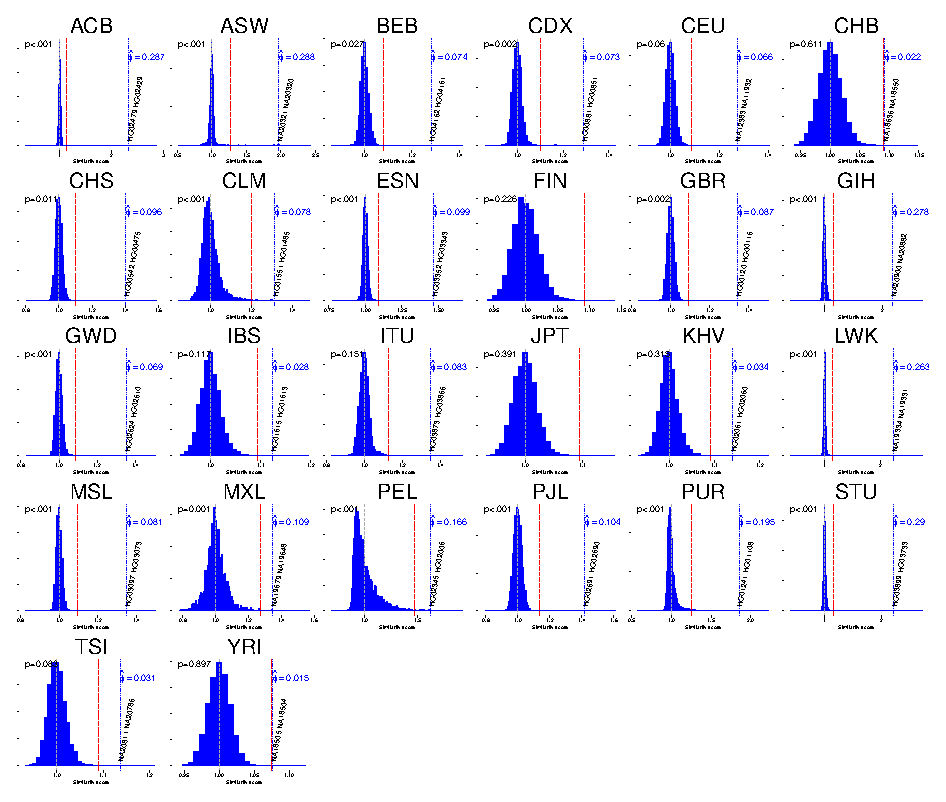
\includegraphics[width=1\linewidth]{figures/figure4}
\caption{\textbf{Differentially involved transcription factors are not necessarily
differentially expressed.} MONSTER commonly finds transcription factors
which are differentially involved but are expressed at similar levels
across cases and controls. This change in involvement suggests that
network rewiring occurs at a post-transcriptional stage. Importantly,
these transcription factors would not have been identified using conventional
differential expression methods.}
\label{fig:expression}
\end{figure}

Our hypothesis is that transcription factors that alter their targets
(and therefore have high $dTFI$ scores) are drivers of changes in
phenotypic state. It would be reasonable to suspect that these transcription
factors would differ across cases and controls at the transcriptional
level. Therefore, we compared $dTFI$ to differential expression in
ECLIPSE (Figure 4, other studies in Supplementary Figure S5). However,
many of the transcription factors with high dTFI were not differentially
expressed in these studies. This suggests that there may be other
mechanisms, including epigenetics, phosphorylation and protein interaction
factors, affecting the structure of gene regulatory networks and that
the master regulators of phenotypic state change may have differentiated
targeting behavior in patients in the COPD group compared to the control
group.

\section*{Discussion}

One of the fundamental problems is biology is modeling the transition
between biological states such as that which occurs during development
or as a healthy tissue transforms into a disease state. As our ability
to generate large-scale, integrative multi-omic datasets has grown,
there has been an increased interest in using those data to infer
gene regulatory networks to model fundamental biological processes.
While there have been many network inference (NI) methods published,
each of which uses a different approach to estimating the \textquotedblleft strength\textquotedblright{}
of interactions between genes (or between transcription factors and
their targets), they all suffer from the same fundamental limitation.
Every method relies on estimating weights that represent the likelihood
of an interaction between two genes to identify \textquotedblleft real\textquotedblright{}
(high confidence) edges.

With MONSTER we acknowledge uncertainty in individual regulatory edgeweights
and instead focus on transcription factor drivers. The effects of
these drivers are more readily apparent when taken over the entirety
of the gene regulatory network. This effectively shines a spotlight
on a reduced search space and thus contributes to the strength of
the findings and reproducibility across studies.

The application of MONSTER to the four studies of COPD demonstrate
the scientific value of the method. Numerous transcription factors
that have been biologically implicated in COPD were found in agreement
across the independent studies. We also demonstrate the utility of
MONSTER by showing that these transcription factors would not have
been detected via differential gene expression analysis or conventional
comparative network inference methods.

Although we apply MONSTER to a set of case-control studies, the method
is not limited to such applications. Our method is suitable in identifying
drivers of state change in any context involving a comparison of gene
expression assays with regulatory data. Given the general nature of
the method, MONSTER has the ability to shed light on possible biological
mechanisms for cell state change that might otherwise have been undetected
in the gene expression data across a wide range of applications.

\subsection*{Supporting Information (SI)}

The main text of the paper must stand on its own without the SI. Refer to SI in the manuscript at an appropriate point in the text. Number supporting figures and tables starting with S1, S2, etc. Authors are limited to no more than 10 SI files, not including movie files. Authors who place detailed materials and methods in SI must provide sufficient detail in the main text methods to enable a reader to follow the logic of the procedures and results and also must reference the online methods. If a paper is fundamentally a study of a new method or technique, then the methods must be described completely in the main text. Because PNAS edits SI and composes it into a single PDF, authors must provide the following file formats only.

\subsubsection*{SI Text}

Supply Word, RTF, or LaTeX files (LaTeX files must be accompanied by a PDF with the same file name for visual reference).

\subsubsection*{SI Figures}

Provide a brief legend for each supporting figure after the supporting text. Provide figure images in TIFF, EPS, high-resolution PDF, JPEG, or GIF format; figures may not be embedded in manuscript text. When saving TIFF files, use only LZW compression; do not use JPEG compression. Do not save figure numbers, legends, or author names as part of the image. Composite figures must be pre-assembled.

\subsubsection*{3D Figures}

Supply a composable U3D or PRC file so that it may be edited and composed. Authors may submit a PDF file but please note it will be published in raw format and will not be edited or composed.

\subsubsection*{SI Tables}

Supply Word, RTF, or LaTeX files (LaTeX files must be accompanied by a PDF with the same file name for visual reference); include only one table per file. Do not use tabs or spaces to separate columns in Word tables.

\subsubsection*{SI Datasets} 

Supply Excel (.xls), RTF, or PDF files. This file type will be published in raw format and will not be edited or composed. 

\subsubsection*{SI Movies}

Supply Audio Video Interleave (avi), Quicktime (mov), Windows Media (wmv), animated GIF (gif), or MPEG files and submit a brief legend for each movie in a Word or RTF file. All movies should be submitted at the desired reproduction size and length. Movies should be no more than 10 MB in size. 

\subsubsection*{Still images}

Authors must provide a still image from each video file. Supply TIFF, EPS, high-resolution PDF, JPEG, or GIF files. 

\subsubsection*{Appendices}

PNAS prefers that authors submit individual source files to ensure readability. If this is not possible, supply a single PDF file that contains all of the SI associated with the paper. This file type will be published in raw format and will not be edited or composed.

\matmethods{Please describe your materials and methods here. This can be more than one paragraph, and may contain subsections and equations as required. Authors should include a statement in the methods section describing how readers will be able to access the data in the paper.  

\subsection*{Subsection for Method}
Example text for subsection.
}

\showmatmethods % Display the Materials and Methods section

\acknow{The project described was supported by Award Number R01 HL089897 and
Award Number R01 HL089856 from the National Heart, Lung, and Blood
Institute. The content is solely the responsibility of the authors
and does not necessarily represent the official views of the National
Heart, Lung, and Blood Institute or the National Institutes of Health. }

\showacknow % Display the acknowledgments section

% \pnasbreak splits and balances the columns before the references.
% If you see unexpected formatting errors, try commenting out this line
% as it can run into problems with floats and footnotes on the final page.
\pnasbreak

% Bibliography
\bibliography{dissertation_research}

\end{document}